\hsection{Text Strings}%
\label{sec:str}%
%
The fourth important datatype in \python\ are text strings.
Text strings are sequences of characters of an arbitrary length.
In \python, they are represented by the datatype \pythonilIdx{str}.
Indeed, we have already used it before, even in our very first example program back that simply printed \pythonil{"Hello World"} in \cref{lst:very_first_program} in \cref{sec:ourFirstProgram}.
\pythonil{"Hello World"} is such a text string.%
%
\hsection{Basic String Operations}%
%
\begin{figure}%
\centering%
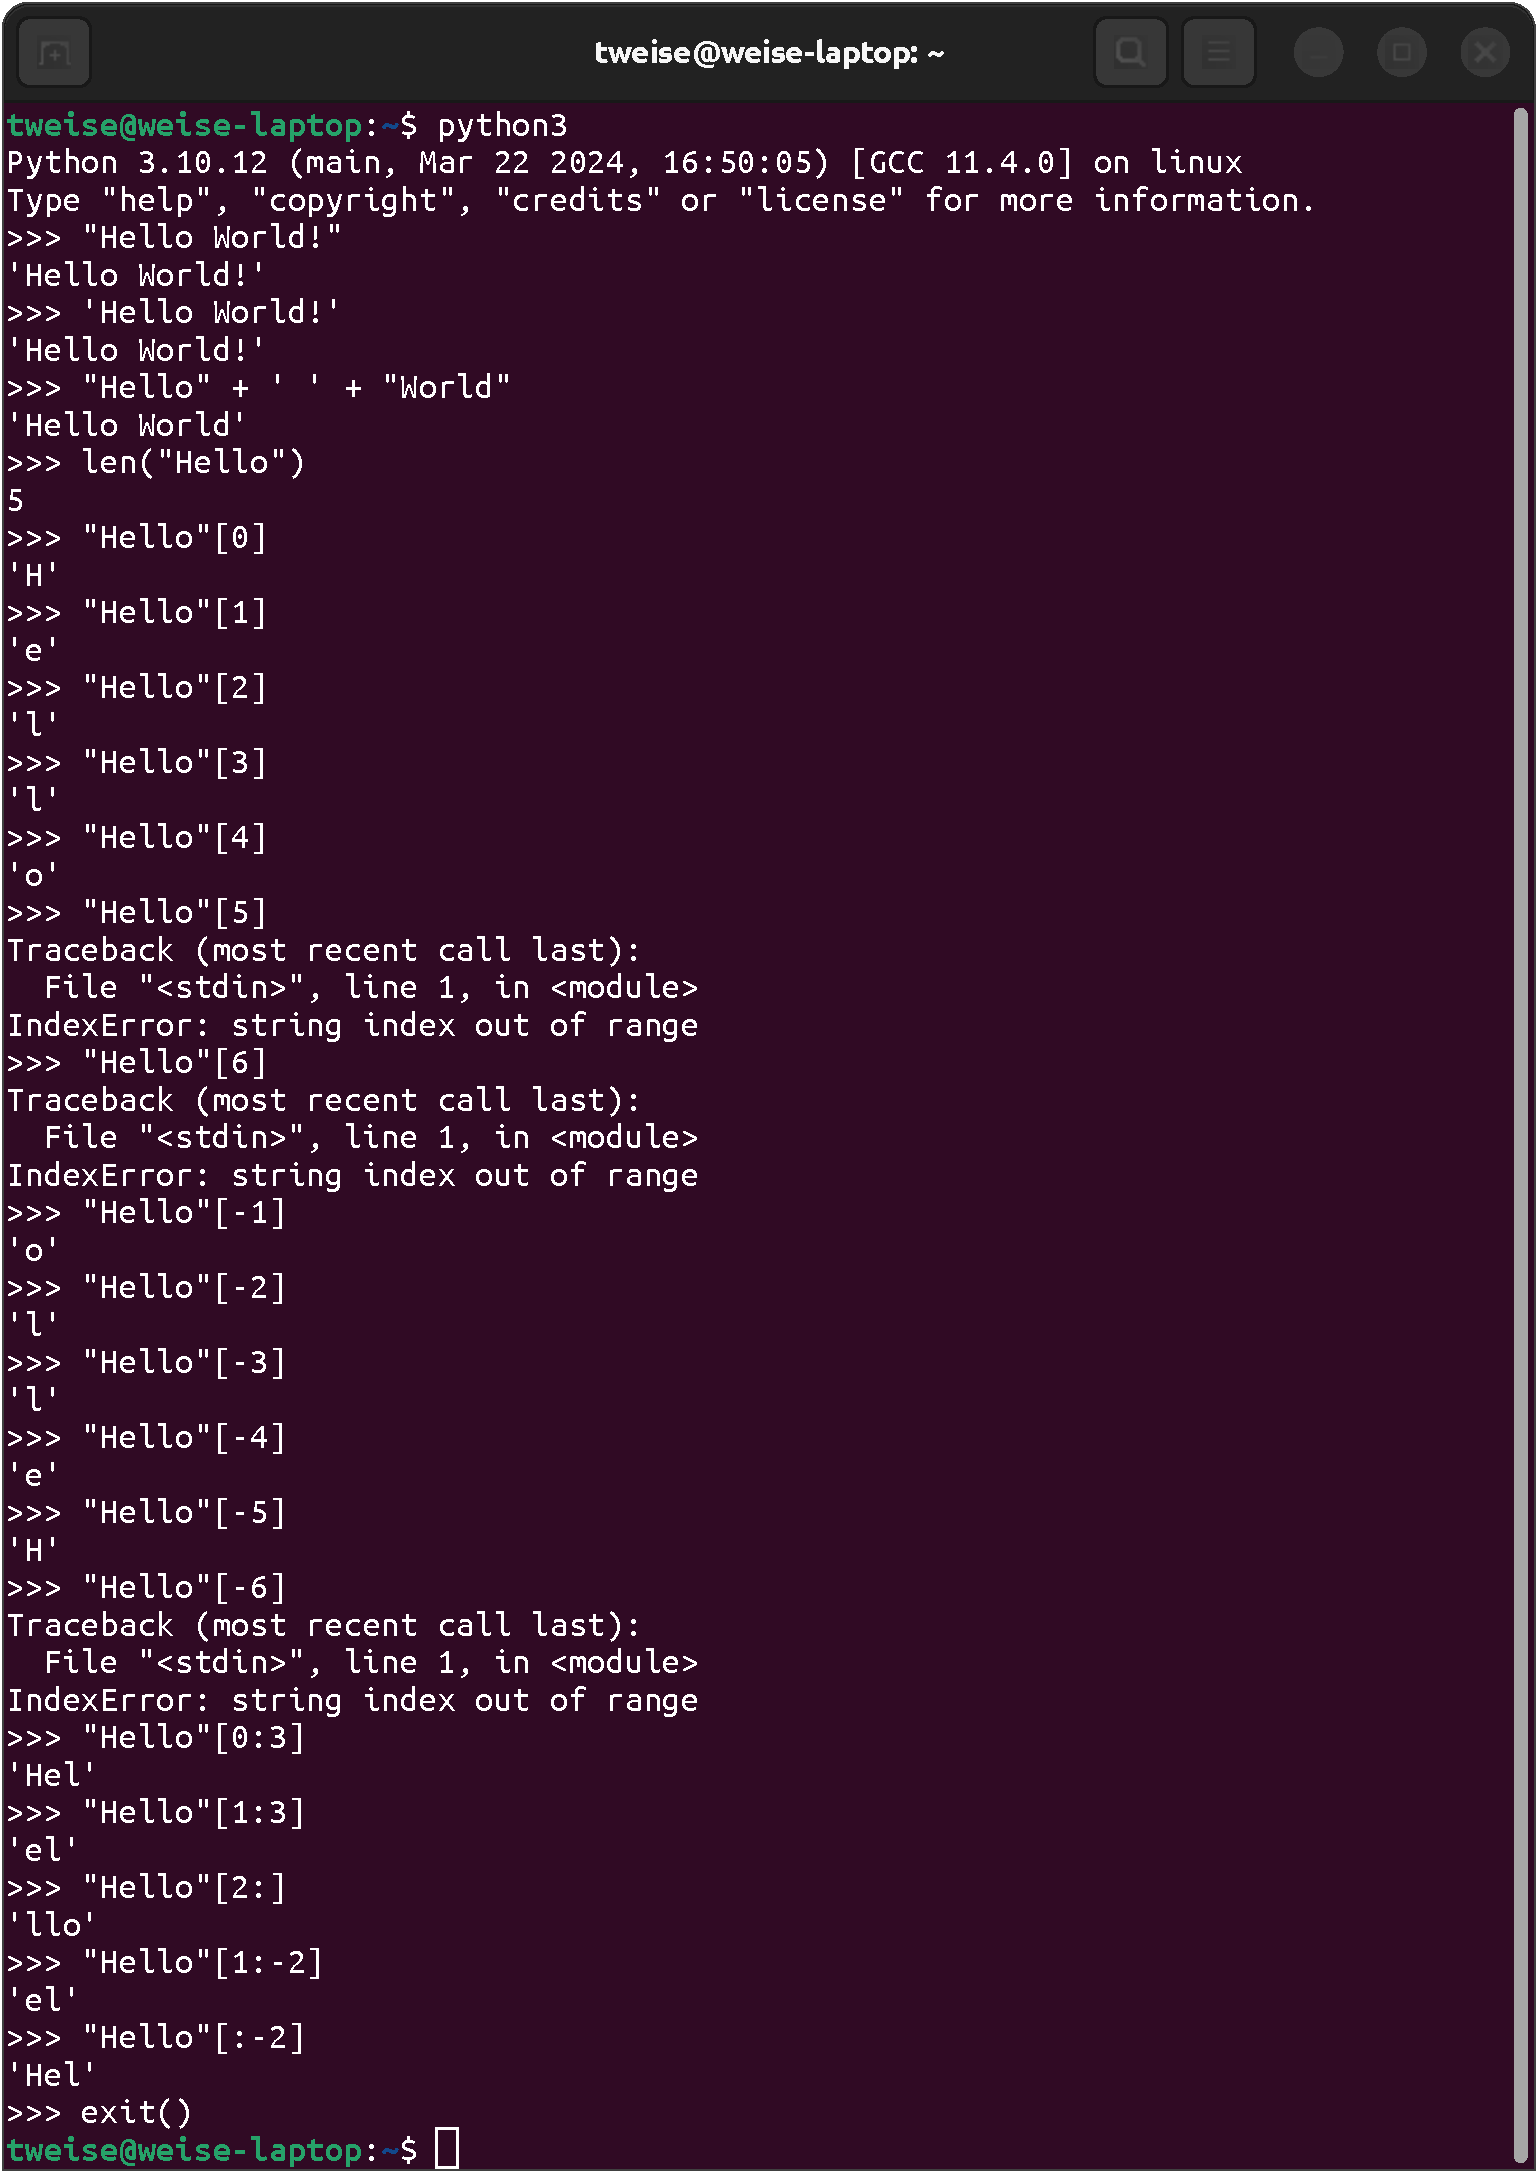
\includegraphics[width=0.8\linewidth]{\currentDir/strIndexing}%
\caption{Specifying string literals and indexing its characters.}%
\label{fig:strIndexing}%
\end{figure}%
%
As \cref{fig:strIndexing} shows, there are two basic ways to specify a text string literal\pythonIdx{str!literal}:
Either enclosed by double quotes, e.g., \pythonil{"Hello World!"}\pythonIdx{\textquotedbl} or enclosed by single quotes, e.g., \pythonil{'Hello World!'}\pythonIdx{\textquotesingle}.
The double-quote variant is usually preferred and we should always use it in our programs.
The quotation marks are only used to delimit the strings, i.e., to tell \python\ where the string begins or ends.
They are not themselves part of the string.

One basic operation is string concatenation\pythonIdx{str!concatenation}\pythonIdx{str!+}\pythonIdx{+}:
\pythonil{"Hello" + ' ' + "World"}\pythonIdx{\textquotedbl}\pythonIdx{\textquotesingle} concatenates the three strings \pythonil{"Hello"}, \pythonil{" "}, and \pythonil{"World"}.
The result is \pythonil{"Hello World"}\pythonIdx{\textquotedbl}.
Notice how the singe space character string is needed, because \pythonil{"Hello" + "World"} would just yield \pythonil{"HelloWorld"}.

Strings are different from the other datatypes we have seen so far.
They are \emph{sequences}\pythonIdx{Sequence}, meaning that they are linear arrays composed of elements.
These elements are the single characters, which correspond to letters, numbers, punctuation marks, white space, etc.

One basic set of things that we can do with strings is to extract these single characters.
First, we need to know the length of a string.
For this purpose, we can invoke the \pythonilIdx{len}\pythonIdx{str!len}\pythonIdx{str!length} function:
\pythonil{len("Hello")} is \pythonil{5}, because there are five characters in \inQuotes{Hello}.
\pythonil{len("Hello World!")} would give us \pythonil{12}, because \pythonil{"Hello"} has five characters, \pythonil{"World!"} has six characters (the \pythonil{"!"} does count!) and there is the single space character in the middle, so $5+6+1=12$.

Knowing the length\pythonIdx{str!length} of a string, we can now safely access its single characters.
These characters are obtained using the square brackets \pythonil{[]}\pythonIdx{str![]}\pythonIdx{[}\pythonIdx{]} with the character index inbetween.
The character indexes start at~0.
Therefore, \pythonil{"Hello"[0]}\pythonIdx{str![]}\pythonIdx{[}\pythonIdx{]} returns the first character of \pythonil{"Hello"} as a \pythonilIdx{str}, which is \pythonil{"H"}\pythonIdx{\textquotedbl}.
\pythonil{"Hello"[1]} returns the second character, which is \pythonil{"e"}.
\pythonil{"Hello"[2]} returns the third character, which is \pythonil{"l"}.
\pythonil{"Hello"[3]}\pythonIdx{str![]}\pythonIdx{[}\pythonIdx{]} gives us the second \pythonil{"l"}.
Finally, \pythonil{"Hello"[4]} gives us the fifth and last character, namely \pythonil{"o"}\pythonIdx{\textquotedbl}.
If we would try to access a character outside of the valid range of the string, say \pythonil{"Hello"[5]}, this results in an \pythonilIdx{IndexError}.
We learn later what errors are and how to handle them -- for now, it is sufficient to know that they will stop your program.
And rightly so, because \pythonil{"Hello"}\pythonIdx{\textquotedbl} has only five characters and accessing the sixth one is not possible and would have an undefined result.

Negative indices, however, are permitted:
The index \pythonil{-1} just means \inQuotes{last character}, so \pythonil{"Hello"[-1]} yields the string \pythonil{"o"}.
The index \pythonil{-2} then refers to the \inQuotes{second-to-last character}, so \pythonil{"Hello"[-2]} gives us \pythonil{"l"}.
The third character from the end, accessed via index \pythonil{-3}, is again \pythonil{"l"}.
\pythonil{"Hello"[-4]} gives us \pythonil{"e"} and \pythonil{"Hello"[-5]} gives us \pythonil{"H"}.
Of course, using a negative index that would bring us out of the string's valid range, such as \pythonil{-6}, again yields an \pythonilIdx{IndexError}.

We can also obtain whole substrings by using index ranges, where the inclusive starting index and the \emph{exclusive} end index are separated by a~\pythonilIdx{:}.
In other words, applying the index \pythonil{[a:b]} to a string results in all characters in the index range from \pythonil{a} to \pythonil{b - 1}.
\pythonil{"Hello"[0:3]} yields a string composed of the characters at positions~0, 1, and~2 inside \pythonil{"Hello"}, i.e., \pythonil{"Hel"}.
The end index is always excluded, so the character at index~3 is not part of the result.
If we do \pythonil{"Hello"[1:3]}, we get \pythonil{"He"}, because only the characters at indices~1 and~2 are included.
If we do not specify an end index, then everything starting at the start index until the end of the string is included.
This means that \pythonil{"Hello"[2:]} will return all the text starting at index~2, which is \pythonil{"llo"}.
We can also use negative indices, if we want.
Therefore, \pythonil{"Hello"[1:-2]} yields \pythonil{"el"}
Finally, we can also omit the start index, in which case everything until right before the end index is returned.
Therefore, \pythonil{"Hello"[:-2]} will return everything from the beginning of the string until right before the second-to-last character.
This gives us \pythonil{"Hel"}.

\begin{figure}%
\centering%
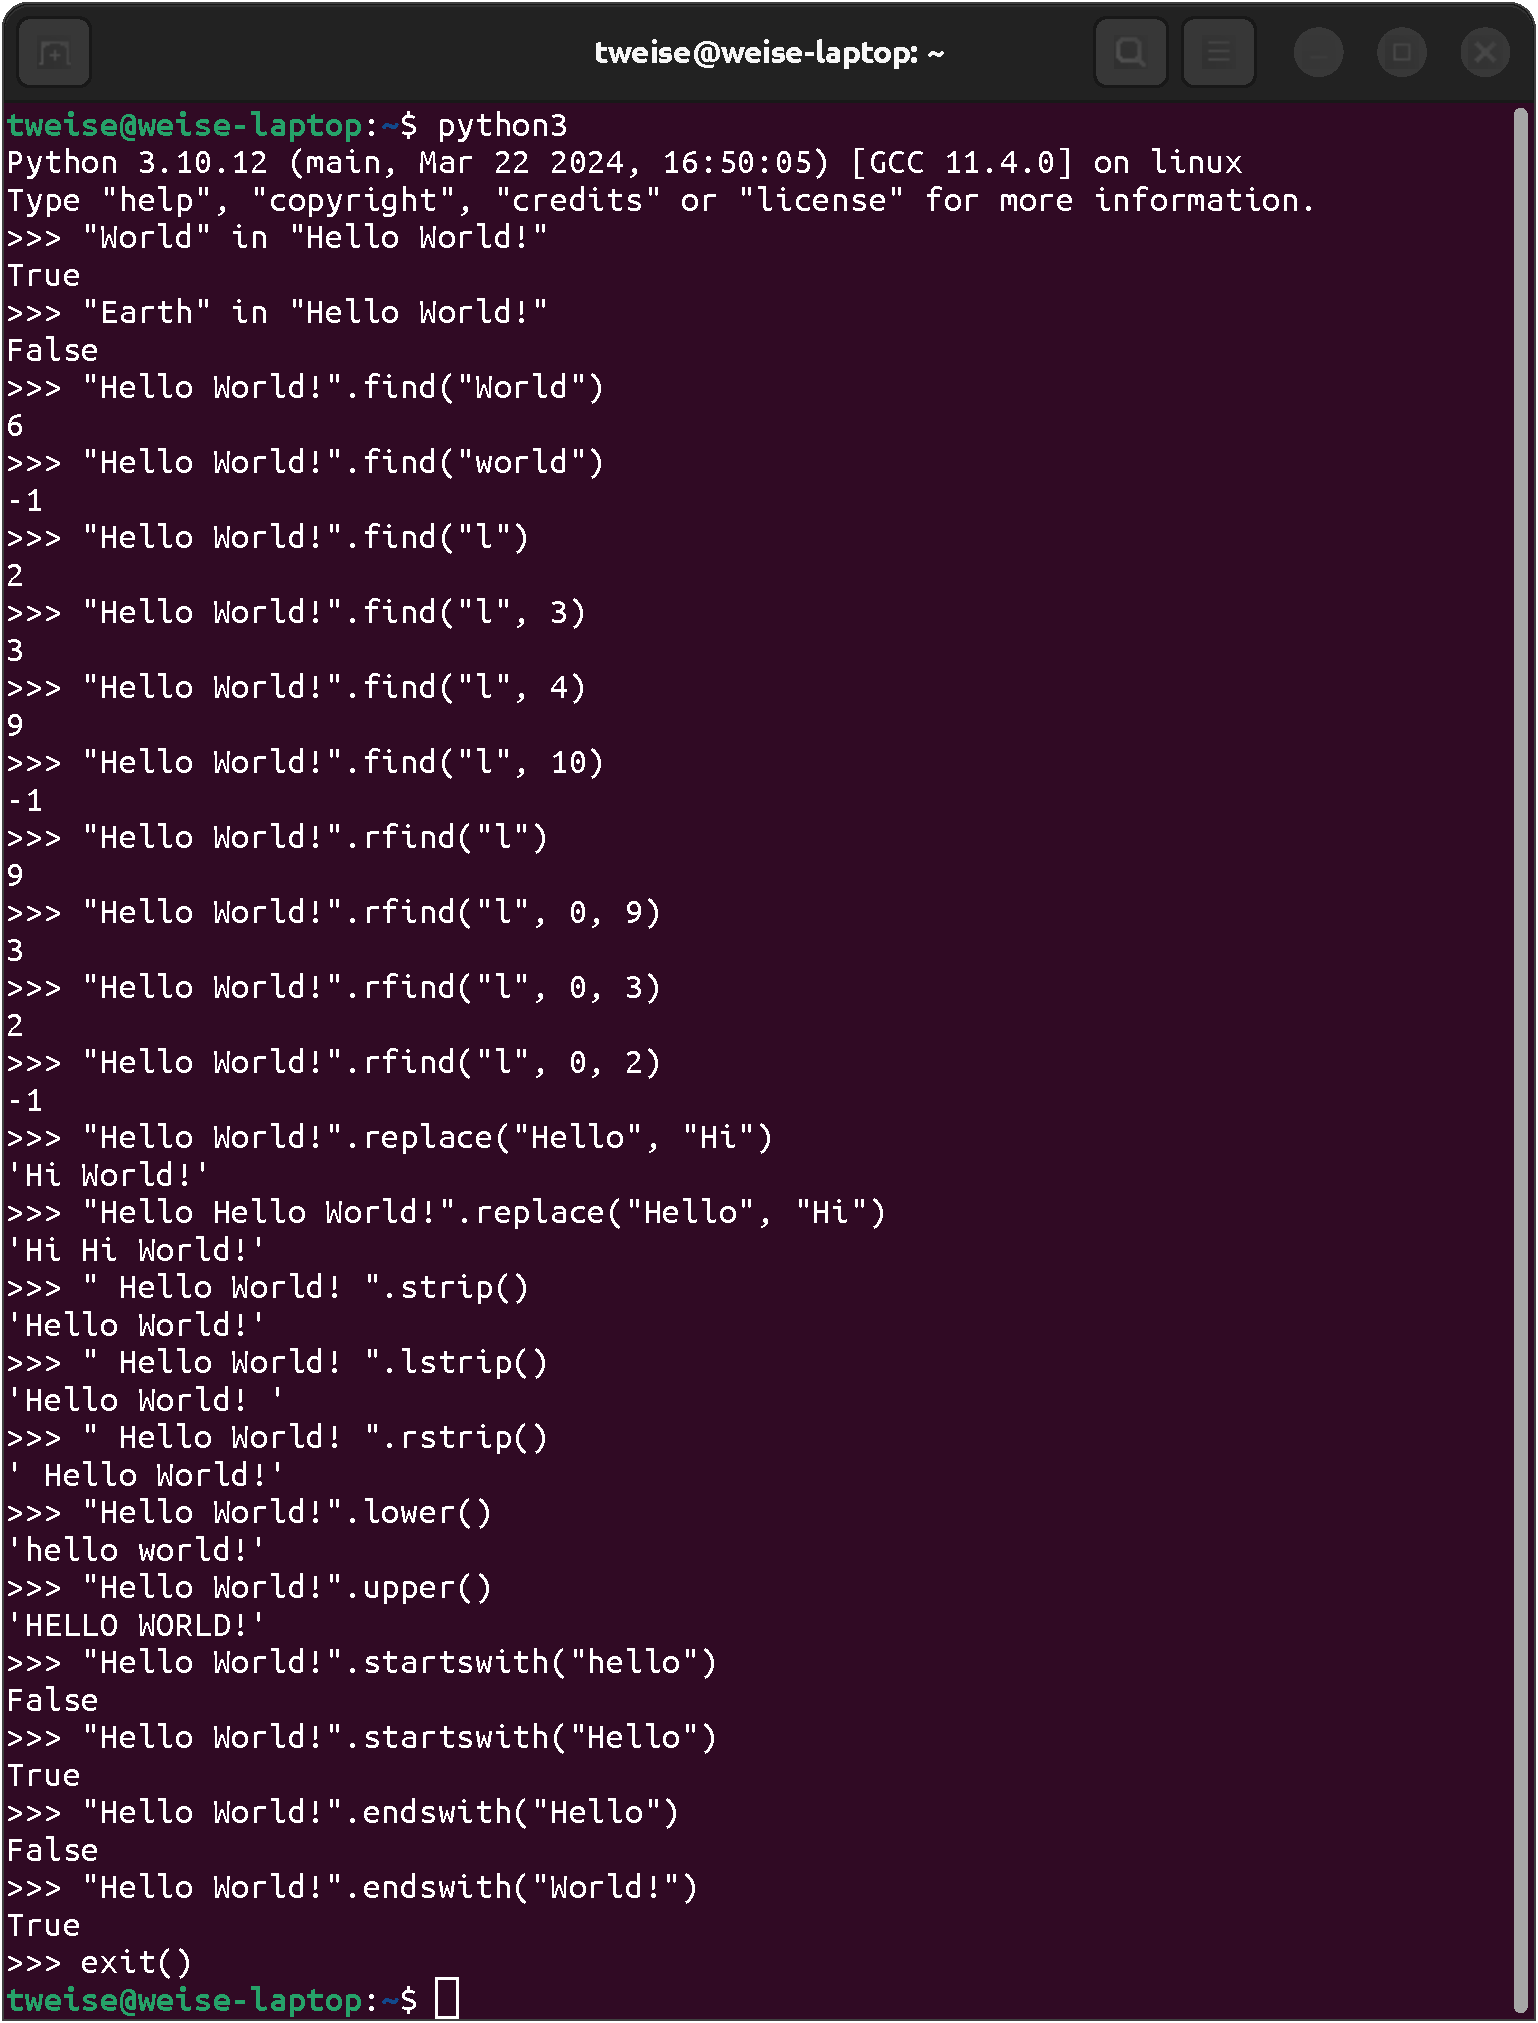
\includegraphics[width=0.8\linewidth]{\currentDir/strBasicOps}%
\caption{Some more basic string operations.}%
\label{fig:strBasicOps}%
\end{figure}%

Besides concatenating and extracting substrings, the \pythonilIdx{str} datatype supports many other operations.
Here, we can just discuss the few most commonly used ones.

There are several ways to check whether one string is contained in another one.
The first method is to use the \pythonilIdx{in} keyword.
As \cref{fig:strBasicOps} shows, \pythonil{"World" in "Hello World!"} yields \pythonilIdx{True}, as it checks whether \pythonil{"World"} is contained in \pythonil{"Hello World!"}, which is indeed the case.
\pythonil{"Earth" in "Hello World!"} is \pythonilIdx{False}, because \pythonil{"Earth"} is not contained in \pythonil{"Hello World!"}.

Often, however, we do not just want to know whether a string is contained in another one, but also \emph{where} it is contained.
For this, the \pythonilIdx{find} method exists.
\pythonil{"Hello World!".find("World")} tries to find the position of \pythonil{"World"} inside \pythonil{"Hello World!"}.
It returns \pythonil{6}, because the \inQuotes{W} of \inQuotes{World} is the seventh character in this string and the indices are zero-based.
Trying to find the \pythonil{"world"} in \pythonil{"Hello World!"} yields~\pythonil{-1}, however.
\pythonil{-1} means that the string cannot be found.
We learn that string operations are case-sensitive\pythonIdx{str!case-sensitive}:
\pythonil{"World" != "world"} would be \pythonilIdx{True}.
We also learn that we need to be careful not to use the result of \pythonilIdx{find} as index in a string directly before checking that it is \pythonil{>= 0}!
As you have learned, \pythonil{-1} is a perfectly fine index into a string, even though it means that the string we tried to find was not found.

Sometimes, the text we are looking for is contained multiple times in a given string.
For example, \pythonil{"Hello World!".find("l")} returns~\pythonil{2}, because \inQuotes{l} is the third character in the string.
However, it is also the fourth character in the string.
\pythonilIdx{find} accepts an optional second parameter, namely the starting index where the search should begin.
\pythonil{"Hello World!".find("l", 3)} begins to search for \pythonil{"l"} inside \pythonil{"Hello World!"} starting at index~3.
Right at that index, the second~\inQuotes{l} is found, so that \pythonil{3} is also returned.
If we search for another~\inQuotes{l} after that, we would do \pythonil{"Hello World!".find("l", 4)}, which returns index~9, identifying the~\inQuotes{l} in~\inQuotes{World}.
After that, no more~\inQuotes{l} can be found in the string, so \pythonil{"Hello World!".find("l", 10)} results in a~\pythonil{-1}.%
%
\begin{sloppypar}%
While \pythonilIdx{find} returns the first occurrence of a string in the supplied range, we sometimes want the last occurrence instead.
If we want to search from the end of the string, we use \pythonilIdx{rfind}.
\pythonil{"Hello World!".rfind("l")} gives us~\pythonil{9} directly.
If we want to search for the~\inQuotes{l} before that one, we need to supply an inclusive starting and exclusive ending index of the range to be searched.
\pythonil{"Hello World!".rfind("l", 0, 9)} searches for any~\inQuotes{l} from index~8 down to~0 and thus returns~\pythonil{3}.
\pythonil{"Hello World!".rfind("l", 0, 3)} gives us~\pythonil{2} and since there is no~\inQuotes{l} before that, \pythonil{"Hello World!".rfind("l", 0, 2)} yields~\pythonil{-1}.
\end{sloppypar}%
%
\begin{sloppypar}%
Another common operation is to replace substrings with something else.
\pythonil{"Hello World!".replace("Hello", "Hi")}\pythonIdx{replace} replaces all occurrences of \inQuotes{"Hello"} in \inQuotes{Hello World} with \inQuotes{Hi}.
The result is \pythonil{"Hi World!"} and \pythonil{"Hello Hello World!".replace("Hello", "Hi")} becomes \pythonil{"Hi Hi World!"}.
\end{sloppypar}%
%
\begin{sloppypar}%
Often, we want to remove all leading or trailing whitespace characters from a string.
The \pythonilIdx{strip} function does this for us:
\pythonil{" Hello World! ".strip()} returns \pythonil{"Hello World!".strip()}, i.e., the same string, but with the leading and trailing space removed.
If we only want to remove the spaces on the left-hand side, we use \pythonilIdx{lstrip} and if we only want to remove those on the right-hand side, we use \pythonilIdx{rstrip} instead.
Therefore, \pythonil{" Hello World! ".lstrip()} yields \pythonil{"Hello World! "} and \pythonil{" Hello World! ".rstrip()} gives us \pythonil{" Hello World!"}.
\end{sloppypar}%
%
In alphabet-based languages, we usually can distinguish between uppercase\pythonIdx{str!uppercase} characters, such as \inQuotes{H} and \inQuotes{W}, and lowercase\pythonIdx{str!lowercase}, such as \inQuotes{e}, \inQuotes{l}, and~\inQuotes{o}.
The method \pythonilIdx{lower} transforms all characters in a string to lowercase and \pythonilIdx{upper} translates them to uppercase instead.
Thus \pythonil{"Hello World!".lower()} returns \pythonil{hello world!} whereas \pythonil{"Hello World!".upper()} yields \pythonil{"HELLO WORLD!"}.

As final functions, we can check whether a string begins or ends with another, we can use \pythonilIdx{startswith} and \pythonilIdx{endswith}, respectively.
\pythonil{"Hello World!".startswith("hello")} is \pythonilIdx{False} whereas \pythonil{"Hello World!".startswith("Hello")} is \pythonilIdx{True}.
\pythonil{"Hello World!".endswith("Hello")} is \pythonilIdx{False}, too, but \pythonil{"Hello World!".endswith("World!")} is \pythonilIdx{True}.

Of course, these were just a small selection of the many string operations available in \python.
You can find more in the \href{https://docs.python.org/3/library/stdtypes.html\#textseq}{official documentation}~\cite{PSF2024TSTS}.%
\endhsection%
%
\hsection{The str Function and f-strings}%
\label{sec:fstrings}%
%
\begin{figure}%
\centering%
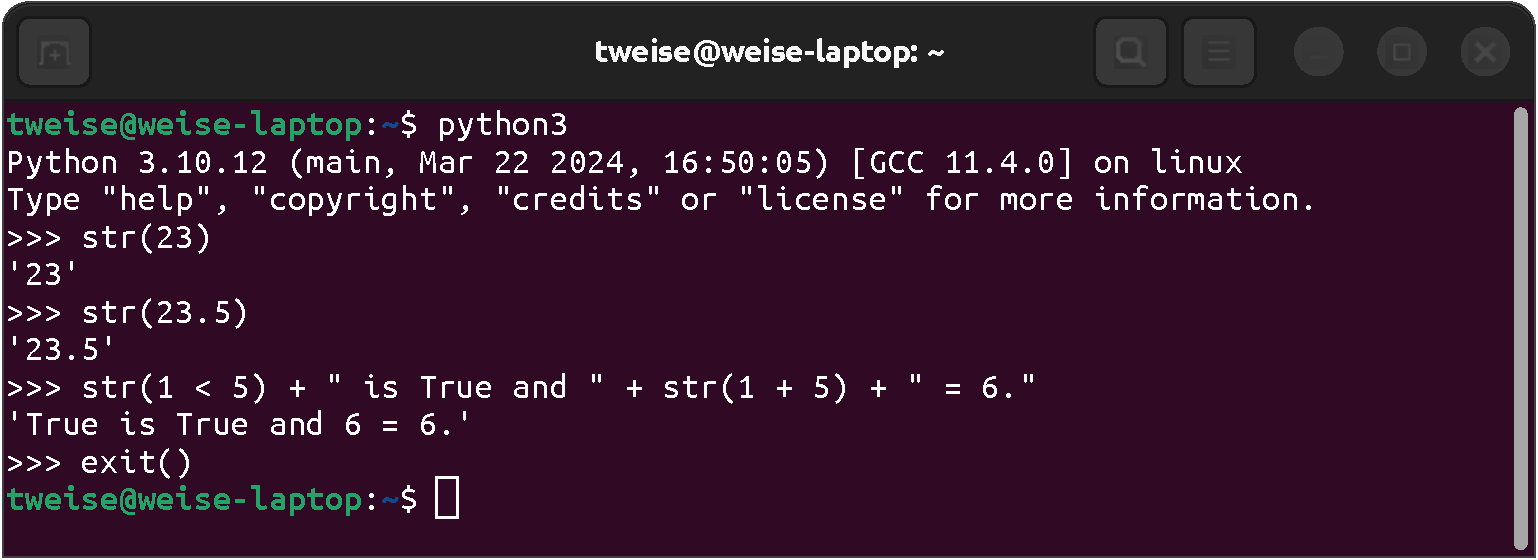
\includegraphics[width=0.8\linewidth]{\currentDir/strStr}%
\caption{The \pythonilIdx{str} function converts objects to strings.}%
\label{fig:strStr}%
\end{figure}%
%
We now have learned the basic operations that can process strings.
However, we did not yet learn one essential thing:
How can we convert an object, like an \pythonilIdx{int} or \pythonilIdx{float} value to a \pythonilIdx{str}?
Very often, we want to perform some complicated calculation that produces a number and then print this number.

In \python, you can convert many different objects to strings by passing them to the function \pythonilIdx{str}\pythonIdx{str!function}.
As \cref{fig:strStr} shows, passing the integer number~\pythonil{23} to \pythonilIdx{str}, i.e., invoking \pythonil{str(23)}, yields the string~\pythonil{"23"}.
Similarly, invoking \pythonil{str} with the \pythonilIdx{float} value \pythonil{23.5} produces the string~\pythonil{"23.5"}.

We can of course concatenate the results of such computations to form more comprehensive texts:
\pythonil{str(1 < 5) + " is True and " + str(1 + 5) + " = 6."} produces \pythonil{"True is True and 6 = 6."}, because \pythonil{1 < 5} evaluated to \pythonilIdx{True}, which is converted to a string, and \pythonil{1 + 5} gives us \pythonil{6}, which, too, is converted to a string.
However, converting data to strings like this is rather tedious.

\begin{figure}%
\centering%
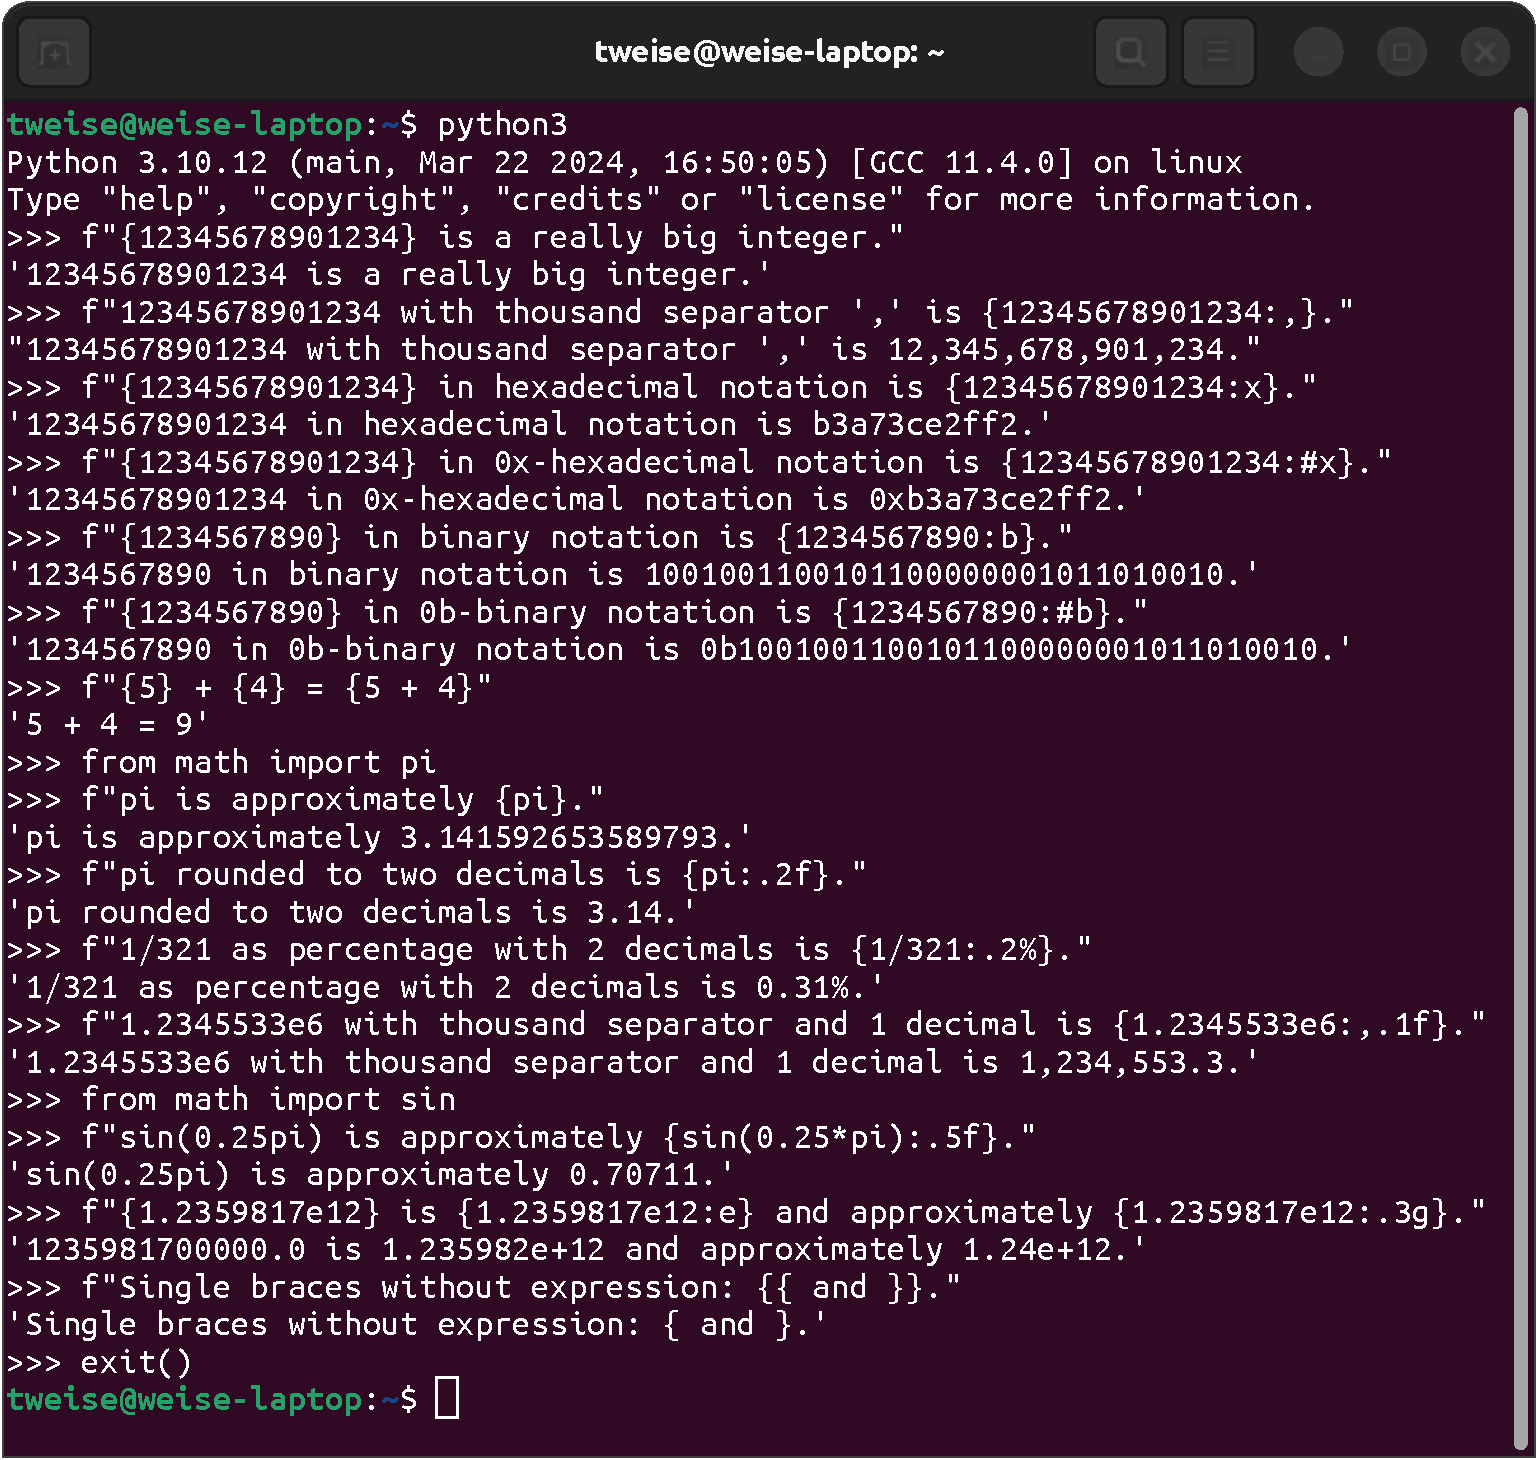
\includegraphics[width=0.8\linewidth]{\currentDir/fstrings}%
\caption{\python\ f-strings in action.}%
\label{fig:fstrings}%
\end{figure}

\pythonIdx{str!f}\pythonIdx{f-string}Let us therefore discuss a very powerful and much more convenient gadget in \python's string processing toolbox: format strings, or \pglspl{fstring}\pythonIdx{f-string}\pythonIdx{str!f} for short~\cite{PSF2024FSL,S2016P4LSI,M2017WAFSIPAHCIUT,B2023PFS}.
An f-string is like a normal string, except that it starts with \pythonil{f"}\pythonIdx{f\textquotedbl} instead of \pythonil{"}.
And, most importantly, it can contain other data and even complete expressions inside curly braces (\pythonil{\{...\}}\pythonIdx{\textbraceleft}\pythonIdx{\textbraceright}) which are then embedded into the string.%
%
\begin{sloppypar}%
In \cref{fig:fstrings}, we first consider the f-string \pythonil{f"\{12345678901234\}\ is a really big integer."}\footnote{
The code that formats my inline \python\ examples sometimes eats spaces after \textbraceleft\ or \textbraceright. %
Therefore, some of the strings presented here may look a bit off. %
In \cref{fig:fstrings}, they are printed correctly, though.}.
This is basically a normal string, except that it contains an integer value.
The opening curly brace~(\inQuotes{\textbraceleft}) right at its beginning signifies that some \python\ expression will begin which must be translated to a string.
The actual expression, \pythonil{12345678901234} is just a really big integer.
The closing curly brace~(\inQuotes{\textbraceright}) signifies the end of the expression.
The \python\ interpreter evaluates all expressions inside such curly braces inside the \pgls{fstring} and then turns their results to strings (and removes the curly braces).
This process is called \emph{\pgls{strinterpolation}}\pythonIdx{f-string!interpolation}\pythonIdx{str!interpolation}.
\pythonil{f"\{12345678901234\}\ is a really big integer."} simply becomes \pythonil{f"12345678901234 is a really big integer."}%
\end{sloppypar}%
%
\begin{sloppypar}%
This first example was not very spectacular.
But \pglspl{fstring} offer us several interesting means to format data.
For example, we can add some formatting specifiers after the expression, separated by~\pythonilIdx{:}.
If our expression evaluates to an \pythonilIdx{int}, then we can specify a \inQuotes{thousand separator} after the~\pythonilIdx{:}.
In western languages, it is usually to group the digits of large numbers in groups of~3.
In Chinese, they tend to use groups of~4 instead.
To the best of my knowledge, we can only specify thousand separators, thought.
This separator will be placed every three digits in the generated text.
As example, \pythonil{f"12345678901234 with thousand separator ',' is \{12345678901234:,\}."} turns into \pythonil{"12345678901234 with thousand separator ',' is 12,345,678,901,234."}.%
\end{sloppypar}%
%
\begin{sloppypar}%
Back in \cref{sec:int:bitstrings}, we learned that integers can also be represented in hexadecimal and binary format.
\pglspl{fstring} conveniently offer this out-of-the-box, we just need to add a~\pythonilIdx{:x} or a~\pythonilIdx{:b} format specifier to the expression, respectively.
For example, the \pgls{fstring} \pythonil{f"\{12345678901234\}\ in hexadecimal notation is \{12345678901234:x\}."} becomes \pythonil{"12345678901234 in hexadecimal notation is b3a73ce2ff2."} and the \pgls{fstring} \pythonil{f"\{1234567890\}\ in binary notation is \{1234567890:b\}."} is turned to \pythonil{"1234567890 in binary notation is 1001001100101100000001011010010."}.
We can also add the \pythonilIdx{0x} and \pythonilIdx{0b} prefixes to the generated number strings by using the \pythonilIdx{:\#x} and \pythonilIdx{:\#b} format specifiers instead.
Let us use the same examples again but instead with the \#-prefixes in the format specifiers.
The hexadecimal variant \pythonil{f"\{12345678901234\}\ in 0x-hexadecimal notation is \{12345678901234:\#x\}."} then becomes \pythonil{"12345678901234 in 0x-hexadecimal notation is 0xb3a73ce2ff2."}.
The binary formatting string \pythonil{f"\{1234567890\}\ in 0b-binary notation is \{1234567890:#b\}."} turns into \pythonil{"1234567890 in 0b-binary notation is 0b1001001100101100000001011010010."}.%
\end{sloppypar}%
%
\begin{sloppypar}%
But \pglspl{fstring} allow us to do even more.
They can contain complete \python\ expressions.
\pythonil{f"\{5\}\ + \{4\}\ = \{5 + 4\}"} is evaluated to \pythonil{"5 + 4 = 9"}.%
\end{sloppypar}%
%
\begin{sloppypar}%
We can also access constants and variables from within the \pgls{fstring}.
Let us again import the constant~$\pi$ from the \pythonilIdx{math} module by doing \pythonil{from math import pi}\pythonIdx{from}\pythonIdx{math}\pythonIdx{import}\pythonIdx{pi}.
We can print it as string by typing \pythonil{f"pi is approximately \{pi\}."} into the \python\ console.
The result is the string \pythonil{"pi is approximately 3.141592653589793."}%
\end{sloppypar}%
%
\begin{sloppypar}%
In many situations, we do not want to see the full \pythonilIdx{float} value with all available significant digits.
We can round it to two decimals by adding the \pythonilIdx{.2f} format specifier.
Three digits would be \pythonilIdx{.3f} and so on{\dots}
Anyway, \pythonil{f"pi rounded to two decimals is \{pi:.2f\}."} gives us \pythonil{"pi rounded to two decimals is 3.14."}.%
\end{sloppypar}%
%
\begin{sloppypar}%
Sometimes, we want to present a floating point value as a percentage.
For example, $\frac{1}{321}=0.003115265\approx0.31\%$.
How can we convert such value to a nice string?
By using the \pythonilIdx{:.2\%} format specifier, which gives us a percentage with two decimals.
\pythonilIdx{:.4\%} would yield three decimals, and so on{\dots}
Therefore \pythonil{f"1/321 as percentage with 2 decimals is \{1/321:.2\%\}."} turns into \pythonil{"1/321 as percentage with 2 decimals is 0.31\%."}.%
\end{sloppypar}%
%
\begin{sloppypar}%
We can also combine thousand separators and rounding to decimals.
The format specifier \pythonilIdx{,.1f} will use the comma~\inQuotes{,} as thousand separator and print a floating point number rounded to one decimal.
The \pgls{fstring} \pythonil{f"1.2345533e6 with thousand separator and 1 decimal is \{1.2345533e6:,.1f\}."} thus is evaluated to \pythonil{"1.2345533e6 with thousand separator and 1 decimal is 1,234,553.3."}.%
\end{sloppypar}%
%
\begin{sloppypar}%
Let us also insert a floating point arithmetic expression in an \pgls{fstring}.
We therefore import the sine function \pythonilIdx{sin} from the \pythonilIdx{math} module via \pythonil{from math import sin}\pythonIdx{from}\pythonIdx{math}\pythonIdx{import}\pythonIdx{sin}.
The \pgls{fstring} \pythonil{f"sin(0.25pi) is approximately \{sin(0.25*pi):.5f\}."} computes the expression \pythonil{sin(0.25*pi)} and presents its result rounded to five decimals via the \pythonilIdx{:.5f} format specifier.
It therefore becomes \pythonil{"sin(0.25pi) is approximately 0.70711."}.%
\end{sloppypar}%
%
\begin{sloppypar}%
We can also use the scientific notation.
The format speciier \pythonilIdx{:e} simply prints a number in scientific notation back from \cref{sec:scientificNotation}.
\pythonilIdx{:.3g} uses scientific notation, but only presents three digits, whereas \pythonilIdx{:.4g} would present four digits, and so on{\dots}
\pythonil{f"\{1.2359817e12\}\ is \{1.2359817e12:e\}\ and approximately \{1.2359817e12:.3g\}."} prints the same number three times.
First, it is simply rendered as normal \pythonilIdx{float} value, then it is rendered in scientific notation, and then it is rendered in scientific notation, but rounded to three digits.
This gives us \pythonil{"235981700000.0 is 1.235982e+12 and approximately 1.24e+12."}.%
\end{sloppypar}%
%
The keen reader may have encountered a question at this stage:
\emph{\inQuotes{What do I do if I want to include a curly brace, say \textbraceleft\ or \textbraceright\ inside my \pgls{fstring}?}}
Well, if you include a single brace, it would be interpreted as start or end of an expression.
If the following text makes sense as expression, it will be interpreted.
If not, an error will occur.
Either way, the curly brace would disappear.
The solution is simple:
If you need \inQuotes{\textbraceleft}, just write \inQuotes{\textbraceleft\textbraceleft}.\pythonIdx{\textbraceleft}\pythonIdx{\textbraceleft\textbraceleft}
It will be interpreted as a single \inQuotes{\textbraceleft}~brace.
If you need \inQuotes{\textbraceright}, just write \inQuotes{\textbraceright\textbraceright}.\pythonIdx{\textbraceright}\pythonIdx{\textbraceright\textbraceright}
It will be interpreted as a single \inQuotes{\textbraceright}~brace.
\pythonil{f"Single braces without expression: \{\{ and \}\}."} simply becomes \pythonil{"Single braces without expression: \{ and \}."}

You are now able to convert the results of your computations to nice text.%
\endhsection%
%
\hsection{Escaping Characters}%
%
\begin{figure}%
\centering%
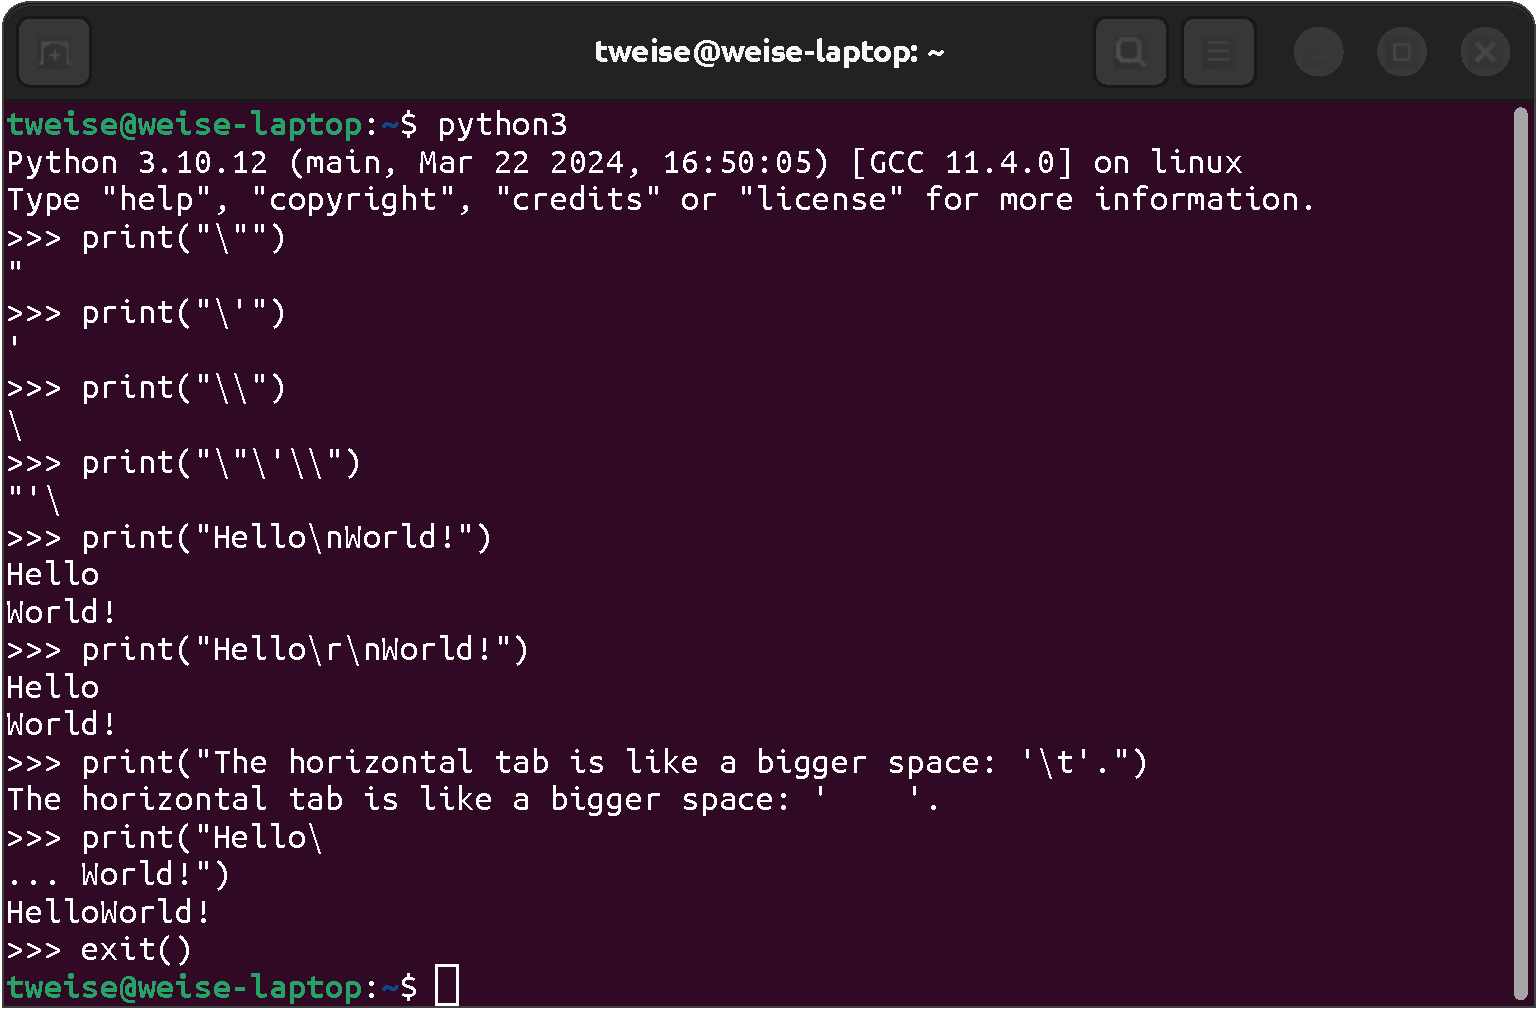
\includegraphics[width=0.8\linewidth]{\currentDir/strEscapes}%
\caption{Escaping special characters in \python\ strings.}%
\label{fig:strEscapes}%
\end{figure}%
%
The last example of \pglspl{fstring} brought up an interesting topic:
\inQuotes{What do we do if we want to use a character in a string which we cannot use?}
For example, if our string is delimited with double quotation marks~\pythonil{"}\pythonIdx{\textquotedbl}, then we cannot put the character \inQuotes{\pythonil{"}} into it, because it would then be interpreted as the end of the string.
On the other hand, if our string is delimited with single quotation marks~\pythonil{'}\pythonIdx{\textquotesingle}, then we cannot put the character \inQuotes{\pythonil{'}} into it, because it would then be interpreted as the end of the string.
Well, you can say, if I need a double quotation mark, then I will delimit my string with single quotation marks and vice versa.
This is all good as long as you do not need \emph{both} single and double quotation marks inside the string.

The answer to this problem is \emph{escaping}\pythonIdx{str!escaping}.
The idea is very simple:
If we need a certain quotation mark, then we simply put a backslash~(\inQuotes{\textbackslash})\pythonIdx{\textbackslash} before it.
The backslash tells the \python\ interpreter that the next character should be considered as a normal character and not be interpreted as any special character, like a string delimiter.

In \cref{fig:strEscapes}, we present several strings with escape sequences.
For clarity reasons, we pass them to the \pythonilIdx{print} function to output them, which means that they show up undelimited in the console.
A double quotation mark can be printed as \pythonil{print("\\"")}, i.e., as a string which is delimited and that then contains the escape sequence {\textbackslash\textquotedbl}\pythonIdx{\textbackslash\textquotedbl}.
It then shows up as~\inlinelistingbox{\texttt{"}} in the output.
A single quotation mark can be printed as \pythonil{print("\\'")}, i.e., via the escape sequence {\textbackslash\textquotesingle}\pythonIdx{\textbackslash\textquotesingle}.
It appears as~\inlinelistingbox{\texttt{'}} in the output.

If the use the backslash character~\inQuotes{\textbackslash}\pythonIdx{\textbackslash} to escape characters which may otherwise have some special meaning {\dots} then what do we do if we need a backslash inside of a string?
Easy: We escape it.
The escape sequence \inQuotes{\textbackslash\textbackslash}\pythonIdx{\textbackslash\textbackslash} is converted to a single backslash and \expandafter\pythonil{print("\\\\")} writes \inlinelistingbox{\texttt{\\}} to the output.
Knowing these sequences, we can now try to \pythonil{print("\\"\\'\\\\")}.
The result printed to the output then is~\inlinelistingbox{\texttt{"'\\}}.

Another situation where escape sequences are nice is when we want to have strings that span over multiple lines.
The newline sequence \inQuotes{\textbackslash{n}}\pythonIdx{\textbackslash{n}} represents a \inQuotes{newline character} which causes the console to skip to the next line.
\pythonil{print("Hello\\nWorld!")} will first print \inlinelistingbox{\texttt{Hello}}, then end the current line and begin a new line, and then print \inlinelistingbox{\texttt{World!}}.
Notice that the newline character sequence \inQuotes{\textbackslash{n}} is used in \linux\ and similar systems, whereas \windows\ uses \inQuotes{\textbackslash{r}\textbackslash{n}}\pythonIdx{\textbackslash{r}\textbackslash{n}}.
Under \python, both always work, regardless under which operating system you are working, and you should \emph{always} use \inQuotes{\textbackslash{n}}.
However, only for the sake of completeness, I include the example \pythonil{print("Hello\\r\\nWorld!")} as well, which produces the same output as \pythonil{print("Hello\\nWorld!")}.

You probably have pressed the tabulator key~\keys{\tab} on your keyboard at some time in the past.
It produces something like a \inQuotes{longer space}.
If you want to include a horizontal tabulator in a string, the escape sequence \inQuotes{\textbackslash{t}}\pythonIdx{\textbackslash{t}} is your friend:
\pythonil{print("The horizontal tab is like a bigger space: '\\t'.")} yields \inlinelistingbox{\texttt{The~horizontal~tab~is~like~a~bigger~space:~'~~~~'.}}.

Finally, a backslash can also escape an actual newline in your string.
If you have a string that is too long to write on a single line but you do not want to have a linebreak inside the actual string, you can simply put a backslash, hit \keys{\enter}, and continue the typing the string.
The linebreak will then be ignored entirely.
Therefore, if you print~\pythonil{print("Hello\\}, hit \keys{\enter}, and then continue to write \pythonil{World!")}, this produces the output~\inlinelistingbox{\texttt{HelloWorld!}}.

Escape sequences allow us to write arbitrary text in strings.
We already leared the sequences \inQuotes{\textbraceleft\textbraceleft}\pythonIdx{\textbraceleft\textbraceleft} and \inQuotes{\textbraceright\textbraceright}\pythonIdx{\textbraceright\textbraceright} that were designed for \pglspl{fstring} only.
The backslash-based escape sequence we discussed in this section work for both \pglspl{fstring} and normal strings.%
\endhsection%
%
\hsection{Multi-Line Strings}%
%
\begin{figure}%
\centering%
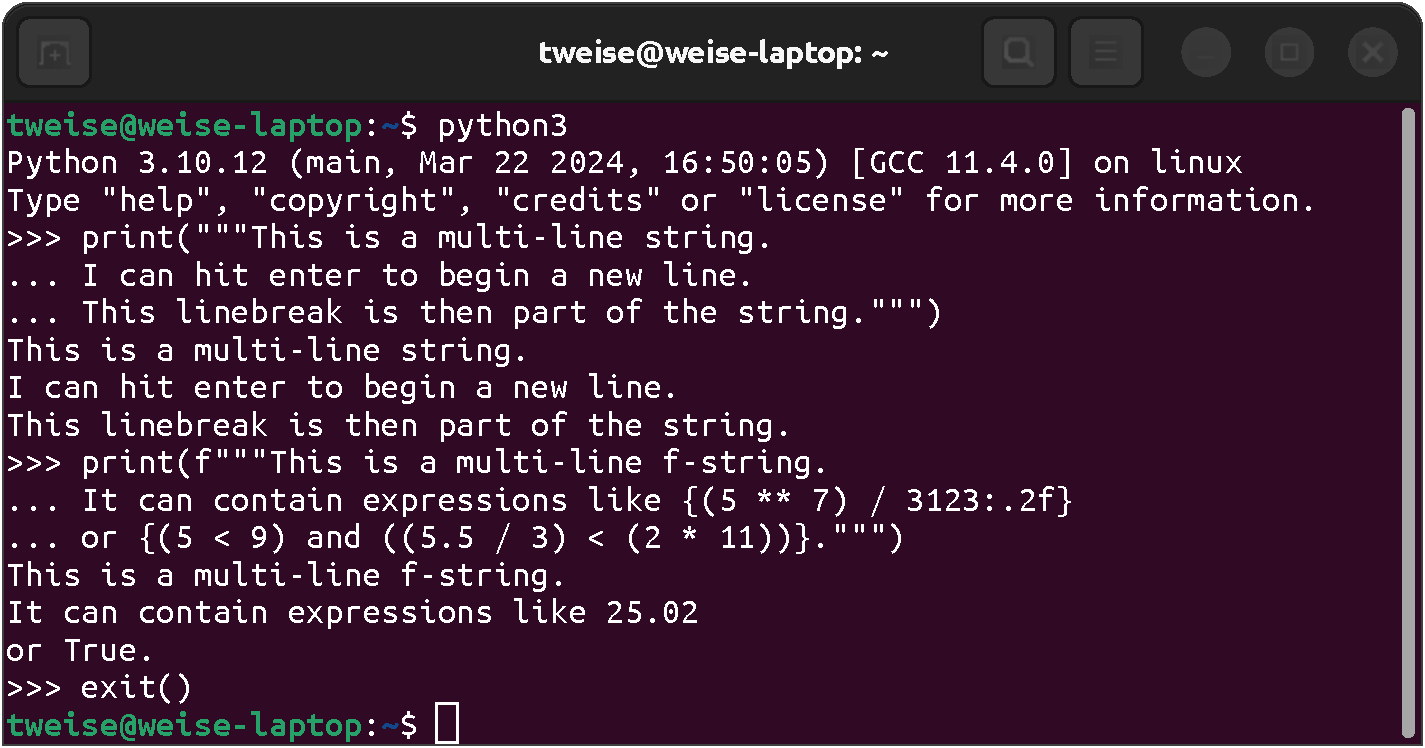
\includegraphics[width=0.8\linewidth]{\currentDir/strMultiline}%
\caption{Examples for multi-line strings.}%
\label{fig:strMultiline}%
\end{figure}%
%
Before we discussed that strings in \python\ are delimited either by \pythonil{"}\pythonIdx{\textquotedbl} or \pythonil{'}\pythonIdx{\textquotesingle} on each side.
However, we can actually delimit them also delimit them with \emph{three quotation marks} on each side, i.e., with either \pythonil{"""}\pythonIdx{\textquotedbl\textquotedbl\textquotedbl} or \pythonil{'''}\pythonIdx{\textquotesingle\textquotesingle\textquotesingle}.
The double quotation mark variant is again preferred.
Such string delimiters are used for multi-line strings.
In such strings, you can insert linebreaks by hitting \keys{\enter} completely normally.
You can use the escape sequences from the previous section as well.
The main use case are docstrings, which we will discuss much later.

\cref{fig:strMultiline} shows what happens if we print such a multi-line string.
We first create the string by writing the three lines \inlinelistingbox{\texttt{This is a multi-line string.}}, \inlinelistingbox{\texttt{I can hit enter to begin a new line.}}, and \inlinelistingbox{\texttt{This linebreak is then part of the string.}}.
The first line begins with \pythonil{"""}\pythonIdx{\textquotedbl\textquotedbl\textquotedbl} and the last one ends with \pythonil{"""}\pythonIdx{\textquotedbl\textquotedbl\textquotedbl} as well.
Passing this text to the \pythonilIdx{print} function, well, prints exactly this three-line string.

We can also have multi-line \pglspl{fstring}\pythonIdx{str!f}\pythonIdx{f-string!multi-line}.
These then simply start with \pythonil{f"""}\pythonIdx{f\textquotedbl\textquotedbl\textquotedbl}.
The example in \cref{fig:strMultiline} presents such a multi-line \pgls{fstring} with two expressions for \pgls{strinterpolation} which spans over three lines.%
\endhsection%
%
\hsection{Unicode and Character Representation}%
%
\noviceHint{%
This section is for readers who want to learn how text is mapped to numbers in order to store it in a computer. %
First-time readers can safely skip over it.}%
%
\begin{figure}%
\centering%
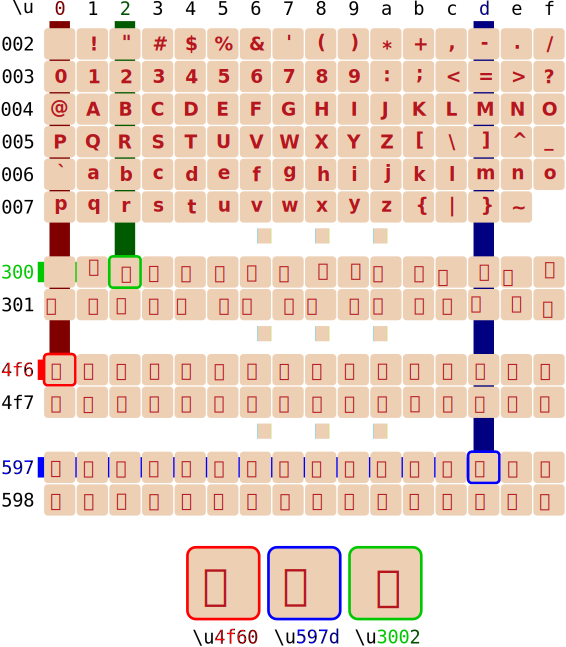
\includegraphics[width=0.65\linewidth]{\currentDir/unicodeCharacterTableSubset}%
\caption{A subset of the \pgls{unicode} character table including the Basic Lating characters as well as some Simplified Chinese characters.}%
\label{fig:unicodeCharacterTableSubset}%
\end{figure}%
%
\begin{figure}%
\centering%
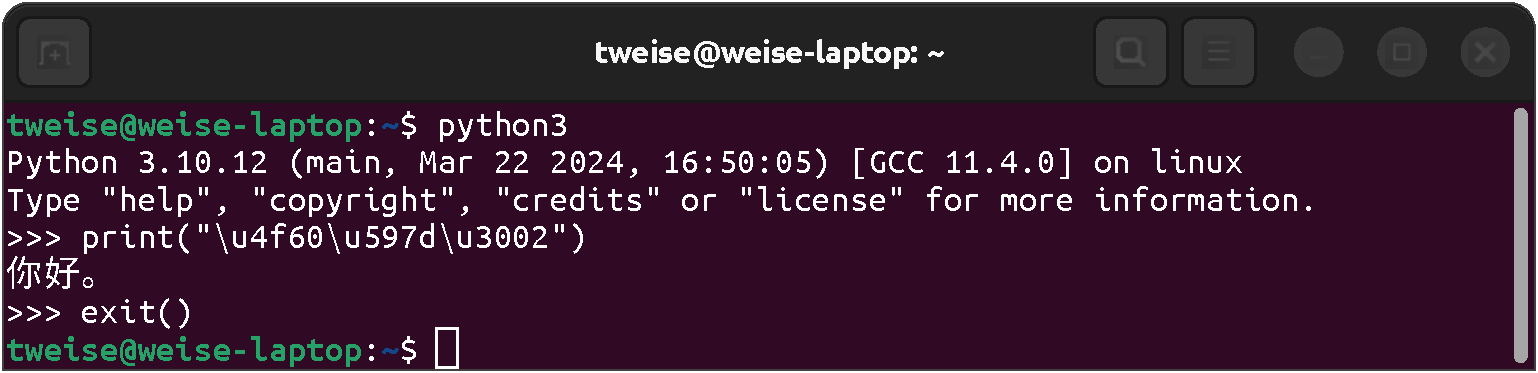
\includegraphics[width=0.65\linewidth]{\currentDir/strUnicodeEscape}%
\caption{\inQuotes{Hello} in Simplified Chinese and entered via \pgls{unicode} escaped string.}%
\label{fig:strUnicodeEscape}%
\end{figure}%
%
The memory of our computers basically stores chunks of bits of certain fixed sizes, say, bytes that are composed of8~bit each.
Usually, these are interpreted as integer numbers.
While \python\ supports arbitrarily large integers, usually we deal with integers composed of 8~bytes, i.e., 64~bits.
The \pythonil{float} datatype in \python\ is also usually 8~bytes large, but these are interpreted differently in order to facilitate fractional numbers (see, e.g., \cref{fig:floatIEEEStructure}).
But how does this work with text?

Well, by mapping characters to numbers.
A \pythonilIdx{str} is then nothing but a list of these numbers.
The system then knows how to interpret these numbers as characters.
Maybe the most well-known historical mapping is ASCII~\cite{ASA1963ASCII,USAS1967USCFII}, which, however, contained only latin characters, punctuation marks, numbers, and some control characters (like the newline and tab characters we learned when discussing string escaping).
Since different languages use different characters, many different mappings have historically evolved and still exist today.
In China, different mappings specialized to Chinese characters exist additionally, including the historical GB~2312~\cite{GBT23121980PROCNSG21CCECSFIE}, GBK~\cite{TSSL1995CICSNSE}, or the newer GB~18030~\cite{GB180302022ITCCCS}.
Today, the vast majority of computers and systems understand one common standard that covers all languages:
\pgls{unicode}~\cite{TUC2023U1510,TUC2023U151ACS,ISOIEC106462020ITUCCSU}, the most frequently used mapping of characters to numbers.
Therefore, \python\ uses \pgls{unicode} as well\pythonIdx{str!unicode}.

\cref{fig:unicodeCharacterTableSubset} illustrates a subset of the \pgls{unicode} code table, including the Basic Latin characters, which are basically still compatible with~ASCII, and some Simplified Chinese characters.
Most \pgls{unicode} characters can be identified by a number represented as four hexadecimal digits (mentioned back in \cref{sec:int:bitstrings}).
The rows \cref{fig:unicodeCharacterTableSubset} are annotated with the first three of these digits and the columns with fourth and last hexadecimal digits.

\python\ allows us to enter \pgls{unicode} characters via a special escape code starting with \pythonil{\\u}\pythonIdx{\textbackslash{u}} followed by these four digits.
This is very useful.
Imagine that you are sharing a program file with some colleagues.
Depending on how their computer encodes text, the Basic Latin characters are usually always interpreted correctly.
But some computers may misinterpret \pgls{unicode} text as something else because the mix up the file encoding.
If we use the \pythonil{\\u}-based\pythonIdx{\textbackslash{u}} escape, then we can represent \emph{any} character as Basic Latin text sequence.
It is also useful if we want to, e.g., enter Chinese text on a machine that does not have an IME or other corresponding tools.

Anyway, in \cref{fig:strUnicodeEscape}, we use the information obtained in \cref{fig:unicodeCharacterTableSubset} to print the Chinese text \inQuotes{Ni Hao.} standing for \inQuotes{Hello.} as unicode escaped string.
We found that the character for \inQuotes{Ni} has unicode number~4f60, \inQuotes{Hao} has~597d, and the big period has~3002.
The string \pythonil{"\\u4f60\\u597d\\u3002"} then corresponds to the correct Chinese text.%
\endhsection%
%
\hsection{Summary}%
Strings, i.e., instances of \pythonilIdx{str}, represent text.
Text is obviously an important element of any program, not just because programs are usually written as text, but because they often receive text as input and send text back as output as well.
Strings are therefore an essential element of programming.
They are basically lists of characters.
We can index them, i.e., extract portions of text, we can search inside a string to check whether and where it contains a certain substring, and we can manipulate strings, e.g., by replacing substrings.

It is also important that we can transform data such as \pythonil{int}s, \pythonil{float}s, or \pythonil{bool}s to strings.
Because we actually \emph{always} print them as strings to the console.
The user cannot interpret the binary representation of such data, they only want text.
While the function \pythonil{str} can convert many different types of objects to strings, we often want to combine several different pieces of information to an output text.
\pglspl{fstring} are the tool for that.
They can render almost arbitrary data as nicely formatted strings and take care of things such as rounding or inserting thousand separators.

Sometimes we want to include characters in our strings that are dodgy.
For example, if our string is delimited by \pythonil{"} marking its begin and end, inserting such a \pythonil{"} inside the string would be awkward.
Indeed, the \python\ interpreter would think that it marks the end of the string and then confuse the \pythonil{"} marking the actual end as the beginning of a new string.
Escape sequences solve this problem:
We would just write \pythonil{\\"} instead of \pythonil{"} if we want to insert a double quotation mark inside a string.
Multi-line strings solve the problem that we sometimes want to enter text as strings that, well, spans multiple lines.

Finally, we learned that strings internally are \pgls{unicode} character sequences.
\pgls{unicode} is a standard that maps the characters of all common languages to numbers.
We can look up the number corresponding to a character in a \pgls{unicode} code table.
Usually, these are four-digit hexadecimal numbers, which we can then use with the special \pythonil{\\u}\pythonIdx{\textbackslash{u}} escape codes in \python.
This allows us to basically represent arbitrary text from arbitrary languages using only the Basic Latin characters.%
\endhsection%
%
\endhsection%
%
